This section surveys related studies first. 
Next, the new hybrid morphological tagging algorithm is described detailing its components and architecture. 
Finally, the presented tool is evaluated through several experiments showing its superior performance.

\subsection{Background}

First of all, we overview how morphological disambiguator systems are typically built up. 
Since there are just a few tools performing full morphological tagging, we also review \gls{pos} tagging attempts for morphologically rich languages. 
In addition, previous Hungarian tagging approaches are introduced as well, hence Hungarian plays an important role in our experiments.

\subsubsection{Full morphological tagging}

There has been insufficient discussion about full morphological tagging in recent studies of natural language technology. 
The reason behind this is that most of the attempts concentrate on morphologically not very rich languages (such as English), where \gls{pos} tagging is generally sufficient and the ambiguity of the lemmatization task is negligible. 
Furthermore, there are studies (following English approaches) which ignore lemmatization (such as~\cite{Hajic1998a,Tufis1998,Silfverberg2011}) even for inflectional languages. 

Nevertheless, studies published on full morphological tagging can be grouped depending on their relationship to lemmatization.

\begin{enumerate}
  \item First of all, numerous researchers propose a two stage model, where the first phase is responsible for finding full morphosyntactic tags, while the second one is for identifying lemmata for \emph{(word, tag)} pairs. 
  For instance, Erjavec and Dzeroski decompose the problem~\cite{Erjavec2004} by utilizing a trigram  tagger first, then applying a decision list lemmatizer. \label{part:general-lemmatization}
  Further on, Agič et al. combine~\cite{Agic2013} an \acrshort{hmm}-based tagger with a data-driven rule-based lemmatizer~\cite{Jongejan}. 
  Even though such combinations could have error propagation issues, they usually result in well-established accuracy.
  \item Another feasible approach is to treat the tagging task as a disambiguation problem. 
  Such methods utilize morphological analyzers to generate annotations candidates, then employ disambiguation methods selecting the correct analyses.
  These architectures are typical e.g. for Turkish attempts (cf.~\cite{Sak2007,Hakkani-Tur2002}).
  %, but similar studies are also published for Czech (such as~\cite{valamelyikHajic}) as well. 
  A drawback of this approach is that the disambiguation components depend heavily on the language-dependent analyzer used.
  \item Finally, the problem can be handled as a unified tagging task.
  A recent study presents the Morfette system~\cite{Chrupaa2008}.
  It employs a joint architecture for tagging words with their tags and lemmata considering lemmatization as a labeling problem.
  Thus, a lemma class is represented as a transformation sequence describing string modifications from the surface form to the root.
  This tool utilizes the \acrshort{maxent} framework employing separate models for each of the subtasks but using a joint beam search decoder.
  A similar method was presented by Laki and Orosz~\cite{Laki2013} recently.
  Their system (HuLaPos) merges \gls{pos} labels with lemmata transformation sequences to a unified tag, which is then learned by the Moses statistical machine translation framework.
  Therefore HuLaPos can \emph{translate} sentences to sequences of labels.
  Such joint approaches are usually language independent, however, they can either be slow or inaccurate due to increased search space.
\end{enumerate}

Considering lemmatization (as in the \ref{part:general-lemmatization}. case), the task can be easily accomplished by using rules or lemma dictionaries, however their creation is time-consuming.
Next, a baseline method is to select the most frequent lemmata for each \emph{(word, tag)} relying on the training data (as in~\cite{zsibrata2013magyarlanc}). 
Despite its simplicity this method usually result in a low precision system.
Further on, employing advanced \gls{ml} algorithms is also a viable approach.
E.g. Plisson et al. apply Ripple Down Rule induction algorithms~\cite{Plisson2004} for learning suffix transformation.
However, their attempt ignores the dependency between tags and lemmata.
Next, Jongejan and Dalianis generate decision lists (cf. CST method~\cite{Jongejan}) for handling morphological changes in affixes.
In that way, their approach explores complex changes in word forms thus being optimized for inflecting languages.  

\subsubsection{Morphosyntactic tagging of morphologically rich languages}

We describe how well-known data-driven \gls{pos} tagging methods are applied for morphologically rich languages focusing on issues yielded by the complexity of the morphology.
Therefore, machine learning models are reviewed investigating techniques applied for managing
\begin{enumerate}
  \item increased number of out-of-vocabulary word forms and
  \item the large complexity of the tagset. 
\end{enumerate}

While numerous attempts have been published for tagging Polish recently~\cite{Piasecki2006,Piasecki2007,Acedanski2010,Radziszewski2013},  performance of such tools presented are below the average.
Most of these solutions (e.g. \cite{Radziszewski2013}) use morphological analyzers to get possible morphosyntactic tag candidates, thus reducing the search space of the decoder.
Further on, tiered tagging is a widely utilized technique~\cite{Radziszewski2013}.
This method resolves complex tags by computing its parts one after another.
Considering \acrshort{ml} algorithms used, the range of applications is wide.
Beside an adaptation of Brill’s tagger~\cite{Acedanski2010}, C4.5 decision trees~\cite{Piasecki2007}, memory-based learning principle~\cite{Radziszewski2011} and \acrshort{crf} models are employed~\cite{Radziszewski2013} as well. 

The first successful attempt to analyze Czech was published by Hajič and Hladká~\cite{Hajic1998a} basing on a discriminative model.
Their approach uses a morphological analyzer and builds on individual prediction models for ambiguity classes.
Actually, the best results for Czech are obtained using the combination of numerous systems~\cite{Hajic2007}.
In their solution, three different stochastic taggers (\acrshort{hmm}, \acrlong{maxent} and averaged perceptron) and symbolic components are utilized as well.
A MA computes the possible analyses, while the rule-based disambiguator tool removes agrammatical tag sequences. 

Besides, the flexible architecture of the Stanford tagger \cite{Toutanova2003} allows the integration of various morphological features enabling its usage for morphologically rich languages.
An example is a Bulgarian tool~\cite{Georgiev2012} by Georgiev et al. which uses a morphological lexicon and an extended feature set.
Beside discriminative models, applications of trigram tagging methods \cite{Brants2000,Halacsy2007} have been demonstrated (for example Croatian~\cite{Agic2013}, Slovenian~\cite{Agic2013} and Icelandic~\cite{Loftsson2007}) to be effective as well.
In contrast with former studies, accurate \acrlong{hmm} based systems usually rely on large morphological lexicons and decent unknown word guessing algorithms.

Considering agglutinative languages with a rich inflectional system, the usage of finite-state methods is indispensable.
Silferberg and Lindén introduce a trigram tagger for Finnish~\cite{Silfverberg2011} relying on a weighted finite-state model.
As regards Turkish, Daybelge and Cicelki describe a system~\cite{Daybelge2007} employing also a finite-state rule-based method.
Most taggers for agglutinative languages use hybrid architectures incorporating morphological analyzers into stochastic learning methods.
Examples are the perceptron based application of Sak et al.~\cite{Sak2007} and the trigram tagging approach of Dilek et al.~\cite{Hakkani-Tur2002}.

To summarize, effective methods for morphologically complex languages rely on either a discriminative or a generative model.
Such taggers generally use morphological lexicons or analyzers to handle the large vocabulary of the target language.
Further on, tagging of unknown words is a crucial problem being managed by either guessing modules or rich morphological features. 

\subsubsection{The case of Hungarian}

As regards Hungarian \gls{pos} tagging, the first attempt was performed by Megyesi~\cite{Megyesi1998} adapting Brill’s transformation based method~\cite{Brill1992}.
Since she did not use any morphological lexicon, her approach resulted in moderate success.
Similarly, Horváth et al. investigated \cite{Horvath1999} only pure machine learning algorithms (such as C4.5 or instance based learning) thus resulting in low accuracy systems.
Three years later, the first promising approach was presented by Oravecz and Dienes~\cite{Oravecz2002a} utilizing TnT~\cite{Brants2000}with a weighted finite-state lexical model.
In 2006, Halácsy et al. investigated an augmented \acrshort{maxent} model~\cite{Halacsy2006} in combination with language specific morphological features and a MA.
In that study, their best result was achieved by combining the latter model with a trigram based tagger.
Later, they created the HunPos system~\cite{Halacsy2007} which reimplements and extends TnT.
Their results (with a morphological lexicon) has been shown to be as efficient as the one of Oravecz and Dienes.
Next, Kuba et al. applied boosting and bagging techniques for transformation based learning.
Although they managed to reduce the error rate of the baseline tagger, their results lag behind previous approaches.
Recently, Zsibrita et al. published \texttt{magyarlanc}~\cite{zsibrata2013magyarlanc}, a natural language processing chain for Hungarian.
They adapted the Stanford \gls{pos} tagger by filtering its suggestions with a morphological analyzer. 

Concerning full tagging involving lemmatization, there are only two methods available for Hungarian.
Although \texttt{magyarlanc} is designed for Hungarian, its lemmatization subsystem is rather simple.
The tool assigns the most common lemmata (depending on the morphosyntactic label) to known words, and employs a rule based unknown word guesser.
Moving on, HuLaPos is applied to Hungarian as well~\cite{Laki2013}, but its performance shown to be dissatisfactory in numerous scenarios. 

This study introduces an accurate morphological tagging method.
We utilize trigram-based \gls{pos} algorithms, since it has superior performance for Hungarian and other agglutinative languages.
The presented tool is adapted for morphologically rich languages and resource-scarce scenarios.
It involves a lemmatization component differing from previous ones yet being competitive with them.
Furthermore, our approach is shown to have state-of-the-art performance for Hungarian while utilizing a language independent hybrid architecture.
In addition, short training time is also guaranteed due to the simple model used.



\subsection{The full morphological tagging model}
\label{sec:purepos}

The architecture of PurePos (cf. Figure \ref{fig:purepos-arch}) contains multiple components. 
The data flow starts from a \gls{ma} providing word analyses as \emph{(lemma, tag)} pairs. 
Next, a trigram model is used to select morphosyntactic labels for words. 
Then, lemmatization is carried out using both statistical and linguistic components. 

\begin{figure}[H]
  \centering
  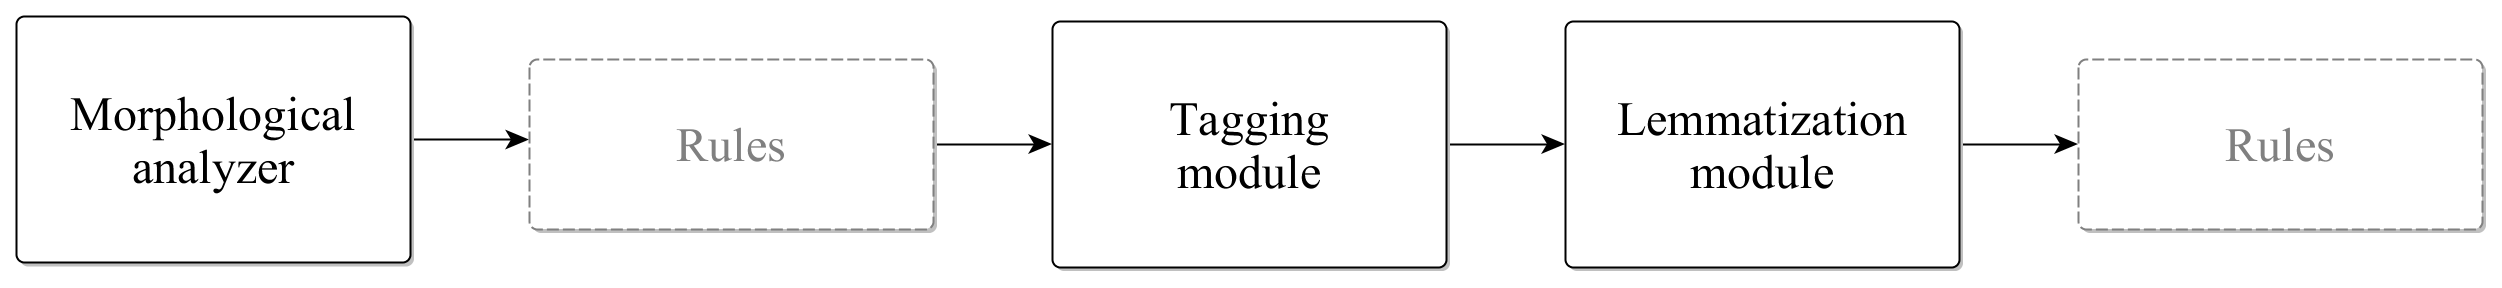
\includegraphics[width=1\textwidth]{MorphTagging/architecture.png} 
  \caption{The architecture of the proposed method}
  \label{fig:purepos-arch}
\end{figure}

In the following, we present the tool's design and components making the morphological tagging effective. 
In that way,  underlying statistical models are introduced first, then we show how symbolic algorithms can be incorporated effectively. 

\subsubsection{The \gls{pos} tagging model}

\begin{figure}[H]
  \centering
  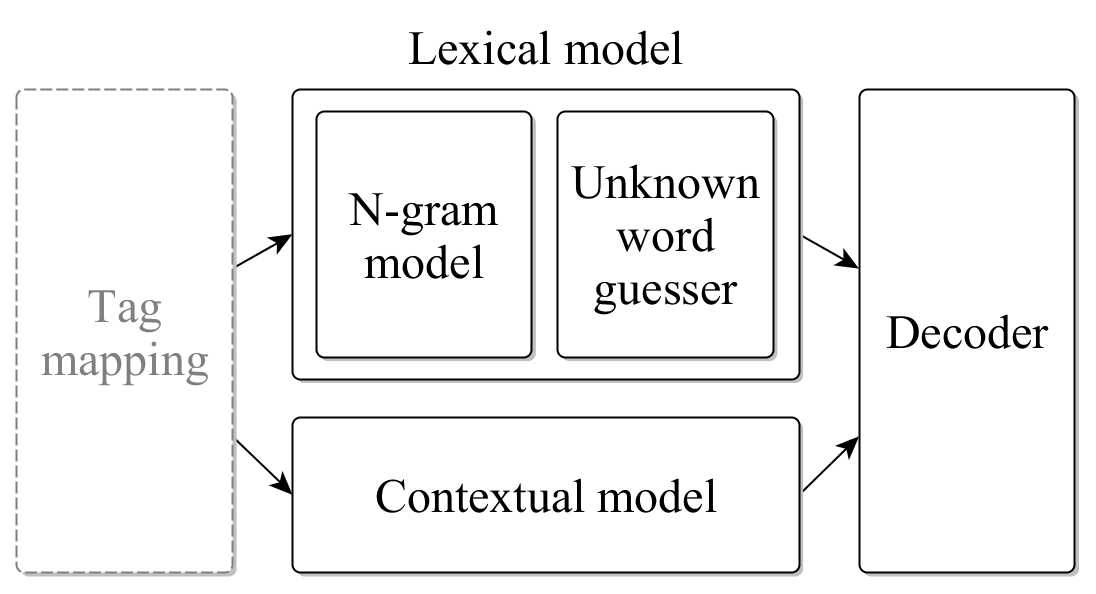
\includegraphics[width=0.5\textwidth]{MorphTagging/pos_arch.png} 
  \caption{The process of part-of-speech tagging in the proposed system}
  \label{fig:pos_arch}
\end{figure}

PurePos builds on \acrshort{hmm}-based methods \cite{Rabiner1989,Samuelsson1993} introduced in TnT \cite{Brants2000}, allowing it to be fast, simple and effective at the same time. 
Similarly to its predecessors, our model (see Figure \ref{fig:pos_arch}) selects the best $t_1 \dots t_m$ label sequence for $w_1 \dots w_n$ words by calculating:
\begin{equation}
\argmax_{t_1^m} \prod_{i=1}^m P(t_i | t_{i-1}^{i-n}) P(w_i|t_{i-1}^{i-n})
\end{equation}

Its contextual model is computed with $n$-gram modeling (cf. Equation \ref{eq:purepos-contextual}) employing \gls{mle} (see Equation \ref{eq:purepos-contextual2})\footnote{Where $N$ denotes the size of the tagset, while $c(x)$ marks the number of $x$ elements in the training data.}. Uni-, bi- and trigram estimates are combined with deleted interpolation thus calculating $\lambda_k$ weights as suggested by Brants \cite{Brants2000}. Even though the order of the model is usually set to 3, it is adjustable in practice. 


\begin{equation}\label{eq:purepos-contextual}
P(t_i | t_{i-1}^{i-n}) = \sum_{k=0}^{n-1} \lambda_k \hat{P}(t_i|t_{i-1}^{i-k})
\end{equation}

\begin{align}\label{eq:purepos-contextual2}
\hat{P}(t_i|t_{i-1}^{i-k}) & = \frac{c(t^{i-k}_i)}{c(t_{i-1}^{i-k})} (k>0) \\
\hat{P}(t_i) & = \frac{c(t_i)}{N} (k=0)
\end{align}

Next, the lexical model of our method \eqref{eq:purepos-lexical} is composed of two components. 
The first one is for tokens previously seen in the training data, while the second guesses labels for unknown words. 
In fact, each subsystem is doubled (as it is in the original study \cite{Brants2000}) maintaining separate models for uppercase and lowercase words. 

Handling of previously seen words is carried out approximating $P(w_i | t_{i}^{i-n})$: 
\begin{equation} \label{eq:purepos-lexical}
P(w_i | t_{i}^{i-n}) = \sum_{k=0}^{n-1} \lambda_k \hat{P}(w_i|t_{i}^{i-k})
\end{equation}

\label{sec:purepos-guesser}
Likewise, \gls{mle} is utilized for estimating $P(w_i|t_{i}^{i-k})$. 
Further on, deleted interpolation is applied using $\lambda_k$ weights. 
Similarly to the contextual model, $k$ is usually set to 2 in applications.

As regards tagging of unknown words, we use -- in accordance with Brants -- the distribution of rare\footnote{Rare words are considered to be those that occur less than 10 times in the training data.}
 tokens’ tags for estimating their \gls{pos} label. Since suffixes are strong predictors for tags in agglutinative languages, we use their ($\{s_{n-l+1} \dots s_n\}$) $l$ long combined frequencies for the guessing process:

\begin{align}
 P(t|s_{n-l+1}, \dots, l_n) 
 = \frac{ \hat{P}(t|s_{n-l+1}, \dots, s_n) + \theta_i \hat{P}(t|s_{n-l}, \dots, s_n)}{1+\theta_i}
\end{align}

In doing so, $\theta_i$ parameters are calculated applying successive abstraction, while \gls{mle} is utilized  again for computing $\hat{P}(t|s_{n-l+1}, \dots, s_n)$. 

Concerning decoding, beam search is utilized, since it can yield multiple tagging sequences at the same time. 
In that way, the tool is able to produce tagging scores of sentences \eqref{eq:purepos-score} allowing us to incorporate linguistic rules building on partly disambiguated word sequences. 

\begin{equation}\label{eq:purepos-score} %%TODO: ez történik, kell ez ide?
Score(w_1^m,t_1^m) = \log \prod_{i=1}^m P(w_i|t_i,t_{i-1})P(t_i|t_{i-1},t_{i-2})P(l_i|t_i,w_i)
\end{equation}

\subsubsection{The lemmatization model}

\begin{figure}[H]
  \centering
  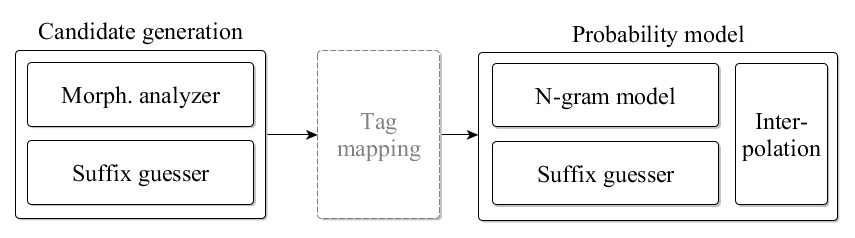
\includegraphics[width=0.8\textwidth]{MorphTagging/lemma_arch.png} %TODO: javítani az ábrán
  \caption{The data flow of the lemmatization component}
  \label{fig:lemma-arch}
\end{figure}

Lemmatization is performed in two steps (cf. Figure \ref{fig:lemma-arch}). 
First, candidates are generated for \emph{(word, morphosyntactic tag)} pairs. 
If morphological analyses are available for the word, their lemmata are used as candidates, otherwise suffix-based guessing is carried out. 
For this, the guesser (described in Section \ref{sec:purepos-guesser}) has been extended to handle lemma transformations as well. 
In doing so, combined labels can represent both the morphosyntactic tag and suffix-transformations for lemmata (for an example see Table \ref{tab:lemma-example}).


\begin{table}[H]
\centering
\caption{Examples for the combined representation of the tag and lemma}
\label{tab:lemma-example}
\begin{tabular}{l | l l}
   \textbf{Word} &  \emph{házam} `my houses’ &  \emph{baglyot} `owl’ \\
   \textbf{Tag} &  \textsc{n.1}s\textsc{pos} &  \textsc{n.acc} \\
   \textbf{Lemma} &  \emph{ház} `house’ &  \emph{bagoly} `owl’ \\
   \textbf{Transformation} & -2+$\varnothing$ &  -4+\emph{oly} \\
   \textbf{Combined label} & (\textsc{n.1}s\textsc{pos}, -2,--) &  (\textsc{n.acc}, -4, \emph{oly}) \\
\end{tabular}
\end{table}


As for picking right lemmata, we utilize a scoring model
\begin{equation}\label{lemma-max}
\argmax_l S(l|t,w)
\end{equation}
for seeking the best lemma for the given token and part-of-speech tag. 
This method is based on the twofold estimation of $P(l|t,w)$. On the one hand, a unigram lemma model ($P(l)$) calculates conditional probabilities using relative frequency estimates. 
On the other hand, reformulation of the core of \eqref{lemma-max} yields another approximation method.


\begin{equation}\label{lemma-guesser}
P(l|t,w) = \frac{P(l,t|w)}{P(t|w)}
\end{equation}

Substituting this formula for the Equation \ref{lemma-max}, $P(t|w)$ becomes a constant which can be omitted. 
In that way, we can estimate $P(l,t|w)$ using the lemma guesser. Finally, models are aggregated in a unified $S$ score applying log-linear interpolation: 


\begin{equation}\label{lemma-interpolated}
S(l|w,t) = P(l)^{\lambda_1} P(l,t|w)^{\lambda_2}
\end{equation}

\begin{algorithm*}
\begin{algorithmic}
    \ForAll{(word, tag, lemma)} 
        \State candidates $\gets$ generateLemmaCandidates(word, tag)
        \State maxUnigramProb $\gets$ getMaxProb(candidates, word, tag, unigramModel)
        \State maxSuffixProb $\gets$ getMaxProb(candidates, word, tag, suffixModel)
        \State actUnigramProb $\gets$ getProb(word, tag, lemma, unigramModel)
        \State actSuffixProb $\gets$ getProb(word, tag, lemma, suffixModel)
        \State unigramProbDistance $\gets$ maxUnigramProb $-$ actUnigramProb
        \State suffixProbDistance $\gets$ maxSuffixProb $-$ actSuffixProb
        \If {unigramProbDistance $>$ suffixProbDistance}
            \State $\lambda_{2} \gets$ $\lambda_{2}$ $+$ unigramProbDistance $-$ suffixProbDistance
        \Else%If{unigramProbDistance $<$ suffixProbDistance}
            \State $\lambda_{1} \gets$ $\lambda_{1}$ $+$ suffixProbDistance $-$ unigramProbDistance
        \EndIf
    \EndFor
    \State normalize$( \lambda_{1}, \lambda_{2} )$
  \end{algorithmic}
  \caption{Calculating parameters of the lemmatization model}
\label{lemma-interpolation-algorithm}
\end{algorithm*}

The idea of computing $\lambda_{1,2}$ parameters is similar to that seen for the \gls{pos} $n$-gram models. 
However, instead of using positive weights, negative scores are stored for the better model.  
It is calculated iterating over words of the training data (cf. Algorithm \ref{lemma-interpolation-algorithm}):
\begin{enumerate}
  \item first, both components return the best lemma assumed for each \emph{(word, tag)} pair, 
  \item then they compute probability estimates for the gold standard lemma,
  \item next, (absolute) error rates of the models are calculated ,
  \item finally, the best model’s weight is decreased.
\end{enumerate}
After these steps, interpolation parameters are normalized.


\subsubsection{Hybridization}

Although the framework proposed builds on an existing \gls{pos} tagging algorithm, it is extended with a new lemmatization model and is modified to fit agglutinative languages such as Hungarian. 
Hybridization steps listed below show differences between PurePos and its predecessors.

\begin{description}
  \item[Morphological analyzer] \hfill \\
  First of all, a morphological analyzer is utilized throughout the whole process estimating probability scores only for valid\footnote{Valid analyses for a word are those which are proposed by the MA.} tags and lemmata.
  \item[Linguistic rules] \hfill \\
  Next, the proposed architecture allows rule-based components to modify the analyses of the MA. In that way, bad candidates can be filtered out. Furthermore, local lexical probability scores can be also given to PurePos, which are then used as context dependent distribution functions. 
  \item[Unseen tags] \hfill \\ 
  In contrast to TnT or HunPos, our system is able to handle unseen tags\footnote{Morphosyntactic labels which are not seen in the training data.} properly. On the one hand, if a token has only one analysis not seen before, that one gets selected with 1 lexical probability. Further on, estimation of forthcoming tags are performed using a lower level (unigram) model in this case. On the other hand, the system can also calculate lexical and contextual scores for any tag previously not seen. This can be performed mapping latter tags to a known ones using regular expressions.\footnote{For a complete example see Section \ref{sec:oldhungarian}.}
  \item[$k$-best output] \hfill \\
  Finally, our method decodes tags using beam search. In doing so, one can generate partly disambiguated sentences being apt for linguistic post-processing. Further on, this facility allows the usage of advanced machine learning techniques resulting in more accurate parsing algorithms.
\end{description}


\subsection{Experiments}

%TODO: ezt a részt átézni
%%%%%%%%%%%%%%%%%%%%%%%%%%%%%%%%%%%%%%%%%%%%%%%%%%%%%%%%%%%%%%%%%%%%%%%%%%%%%%%%%%%%%%%%%%%%%%%%%%%%%%%%%%%%%%%%%%%%%%%%

\subsubsection{Tagging general Hungarian}

First, PurePos is evaluated on Hungarian using the Szeged Corpus\footnote{Version 2.3 is utilized in our experiments, since the MA employed is only compatible with this corpus variation.}~\cite{Csendes2004} (SZC). 
This corpus contains general texts from seven genres being annotated with detailed (MSD) morphosyntactic tags~\cite{Erjavec2012} and lemmata.
In addition, we used a variant of the same corpus tagged with the analyses of the Humor MA. These texts were split in 8:2 ratio for training and testing (as in Table \ref{tab:szeged-corpus}). 

\begin{table}[H]
\centering
\caption{Dimensions of the corpora used}
\begin{tabular}{l r r r r}
  \hline
  & \multicolumn{2}{c}{MSD tagset} & \multicolumn{2}{c}{Humor tagset} \\
  &  Training set &  Test set &  Training set &  Test set  \\
  \hline
  Tokens &  1,232,384 &  254,880 &  980,225 &  214,123 \\
  Sentences &  68,321 &  13,778 &  56,792 &  14,198 \\
  Distinct tags &  1,032 &  716 &  983 &  656 \\
  \hline
\end{tabular}
\label{tab:szeged-corpus}
\end{table}

As a morphological analyzer is an integral part of our method, we tested the tool with two analyzers. 
The first setting utilizes the MSD tagged corpus and an analyzer extracted from \texttt{magyarlanc}, while the second one applies Humor with the transcribed corpus.

Evaluation is carried out measuring the overall precision of full annotations (i.e \emph{(morphosyntactic tag, lemma)} pairs). 
Further on, sentence-based accuracies are also provided in some cases. 
The latter metric is computed by considering a sentence to be correct only when all of its tokens are properly tagged. 

Further on, morphological tagging tools available for Hungarian were also evaluated. 
Firstly, \texttt{magyarlanc}, HuLaPos and Morfette\footnote{Version 3.5 is used.} are compared with PurePos.  
%Next, combination of lemmatization and \gls{pos} tagging tools are investigated. 
Two-phase architectures have been shown to be prosperous (e.g.~\cite{Agic2013,Erjavec2004}) for several scenarios, therefore successful modules being commonly applied are also involved in our experiments. 
Concerning \gls{pos} taggers, we use
\begin{itemize}
  \item the trigram tagging method of HunPos,
  \item averaged perceptron learning and
  \item the maximum entropy framework of the OpenNLP~\cite{Baldridge2002} toolkit.
\end{itemize}

As regards lemmatization tools, CST and a baseline method are employed. 
The latter one results on roots for \emph{(word, tag)} pairs being the most frequent in the training data. 
Beside these components, tag dictionaries have been prepared for HunPos. 
(For this, morphological analyzers are fed with the 100 000 most frequent words of Hungarian\footnote{Frequencies are calculated relying on the results of the Szószablya project~\cite{Halacsy2004}.}.) %TODO: ez tuti az?

\begin{table}[H]
 \centering
 \caption{Morphological tagging precision scores on the Szeged Corpus (annotated with MSD labels)}
\begin{tabular}{l r r r}
  \hline
  Precision &  PoS tag &  Token &  Sentence \\
  \hline
  \texttt{magyarlanc} &  96.50\% &  95.72\% &  54.52\% \\
  Morfette &  96.94\% &  92.24\% &  38.18\% \\
  HuLaPos &   &   &   \\
  PurePos &  \underline{96.99\%} &  \underline{96.27\%} &  \underline{58.06\%} \\
  HunPos + BL &  96.71\% &  92.65\% &  36.06\% \\
  HunPos + CST &  96.71\% &  91.19\% &  35.31\% \\
  Maxent + BL &  95.63\% &  92.21\% &  34.82\% \\
  Maxent + CST &  95.63\% &  90.14\% &  29.70\% \\
  Perceptron + BL &  95.19\% &  91.16\% &  29.42\% \\
  Perceptron + CST &  95.19\% &  89.78\% &  27.91\% \\
  \hline
\end{tabular}
\label{tab:morphtag-orig}
\end{table}


\begin{table}[H]
 \centering
 \caption{Morphological tagging precision scores on the transcribed Szeged Corpus (annotated with Humor labels)}
\begin{tabular}{l r r r}
  \hline
  Precision &  PoS tag &  Token &  Sentence \\
  \hline
  Morfette &  97.60\% &  94.73\% &  51.58\% \\
  HuLaPos &   &   &   \\
  PurePos &  \underline{98.65\%} &  \underline{98.58\%} &  \underline{81.78\%} \\
  HunPos + BL &  97.41\% &  89.93\% &  32.07\% \\
  HunPos + CST &  97.41\% &  94.69\% &  52.40\% \\
  Maxent + BL &  94.81\% &  88.82\% &  28.19\% \\
  Maxent + CST &  94.81\% &  92.33\% &  40.10\% \\
  Perceptron + BL &  95.97\% &  88.85\% &  29.11\% \\
  Perceptron + CST &  95.97\% &  93.32\% &  45.13\% \\
  \hline
\end{tabular}
\label{tab:morphtag-humor}
\end{table}


First of all, there are notable discrepancies of the results on the two datasets. 
On one hand, these can be explained by the different annotation scheme they use:
\begin{itemize}
  \item First, the original corpus contains foreign and misspelled words being tagged with a uniform \textsc{x} tag. Due to the various syntactic behavior of such words, their labels can be hardly estimated using their context or their suffix.
  \item Further on, date expressions and several named entities are tagged with a single MSD code resulting in lemmata composed of more than one word. (An example is \emph{Golden Eye-oztunk} `we visited the Golden Eye’ being lemmatized as \emph{Golden Eye-ozik} `to visit the Golden Eye’.) 
  Such phenomena could be hard to handle for lemmatizers.
\end{itemize}
Such differences affect morphological disambiguation algorithms significantly, thus decreasing the accuracy of MSD-based systems.
However, the Humor-tagged corpus is free of such words, thus allowing taggers to produce better annotation. 
On the other hand, morphological analyzers differ by their coverage affecting performance of parsing chains built on them.

Results in Tables \ref{tab:morphtag-orig} and \ref{tab:morphtag-humor} show that PurePos is the most accurate tool for Hungarian. 
First, it is very effective on \gls{pos} tagging. % thanks to the morphological analyzers used. 
Next, comparison of full annotation scores reveals that the new lemmatization algorithm significantly outperforms others. 

As regards the MSD-tagged corpus, \texttt{magyarlanc} yields first-class results with a precision of 95.72\%, however, its language specific components inhibits its application on other corpora. 
Further on, the performance of Morfette and HuLaPos are still prosperous, but they yield significantly worse accuracy than that of PurePos.  

It has been also found that two-stage taggers are far behind state-of-the-art results. 
Even though, the \gls{pos} accuracy of HunPos is close to the best ones, both of the standalone lemmatizers degrade the overall performance. 
This is due to the fact that the baseline method could have difficulties with unknown words, while CST was originally designed for inflectional languages. 

Finally, sentence based accuracies on the Humor-tagged corpus reveals that most of the tools result in erroneously tagged sentences in more than half of the cases, while the same number for PurePos is less than 20\%. Furthermore, its lemmatization method outperforms all other systems available for Hungarian.



\subsubsection{Resource-scarce settings}

Next, we show that our method, in contrast to others (see methods investigated in the previous section\footnote{Unfortunately, we could not measure the performance of \texttt{magyarlanc}, since the current release of the tool cannot be trained.}), can be used effectively when just a small amount of annotated corpora is available. 
For this, we draw learning curves of systems, evaluating them on the same datasets. 
However, data used for training is limited to 2,000, 4,000, 6,000, 8,000 and 10,000 sentences. 

\begin{figure}[H]
  \centering
  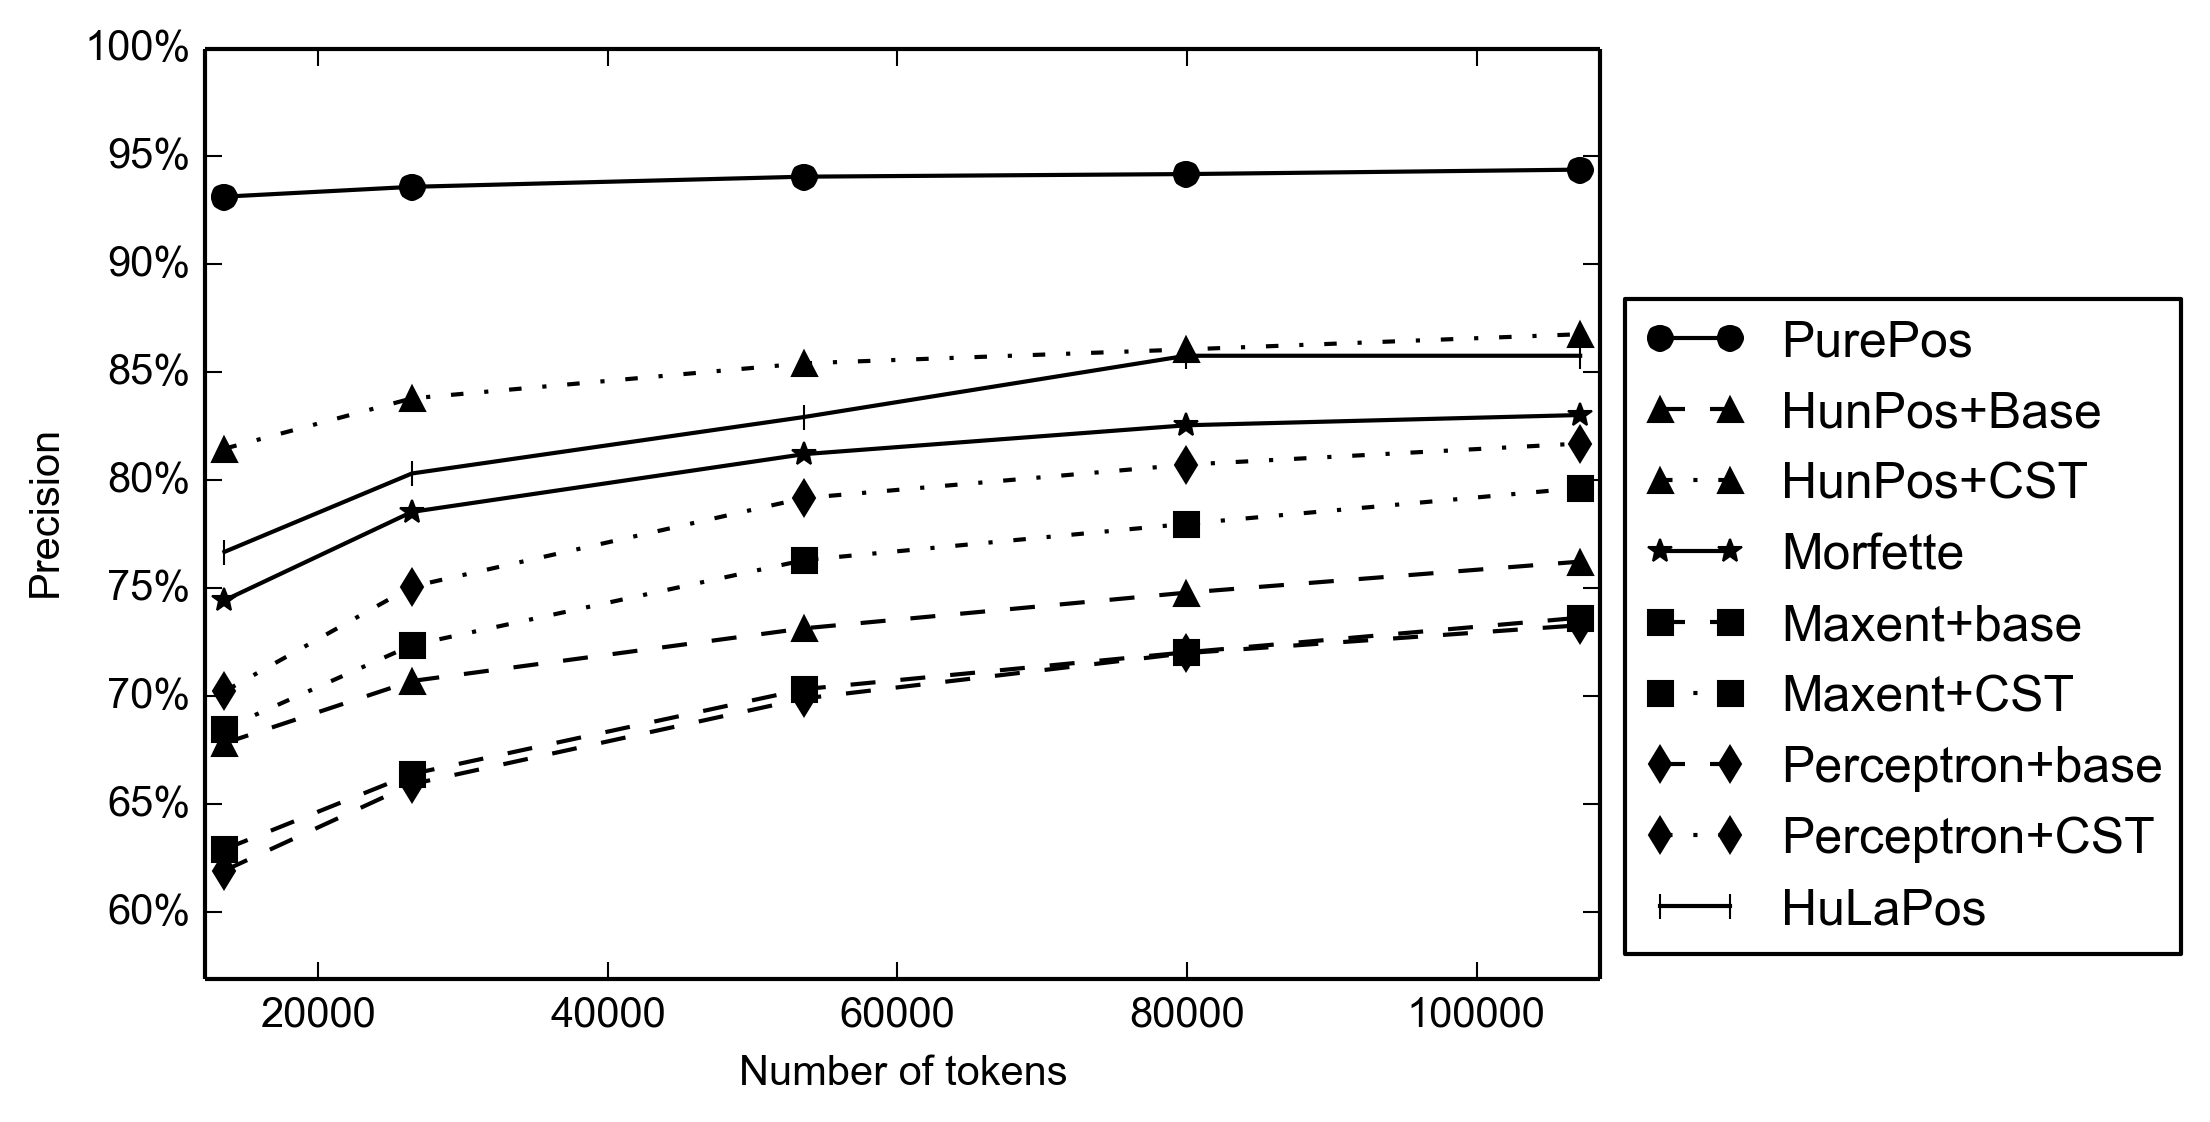
\includegraphics[width=1\textwidth]{MorphTagging/msd_token.png} 
  \caption{Learning curves (regarding token accuracy) of full morphological taggers on the Szeged Corpus (using MSD labels)}
  \label{fig:msd-token}
\end{figure}

\begin{figure}[H]
  \centering
  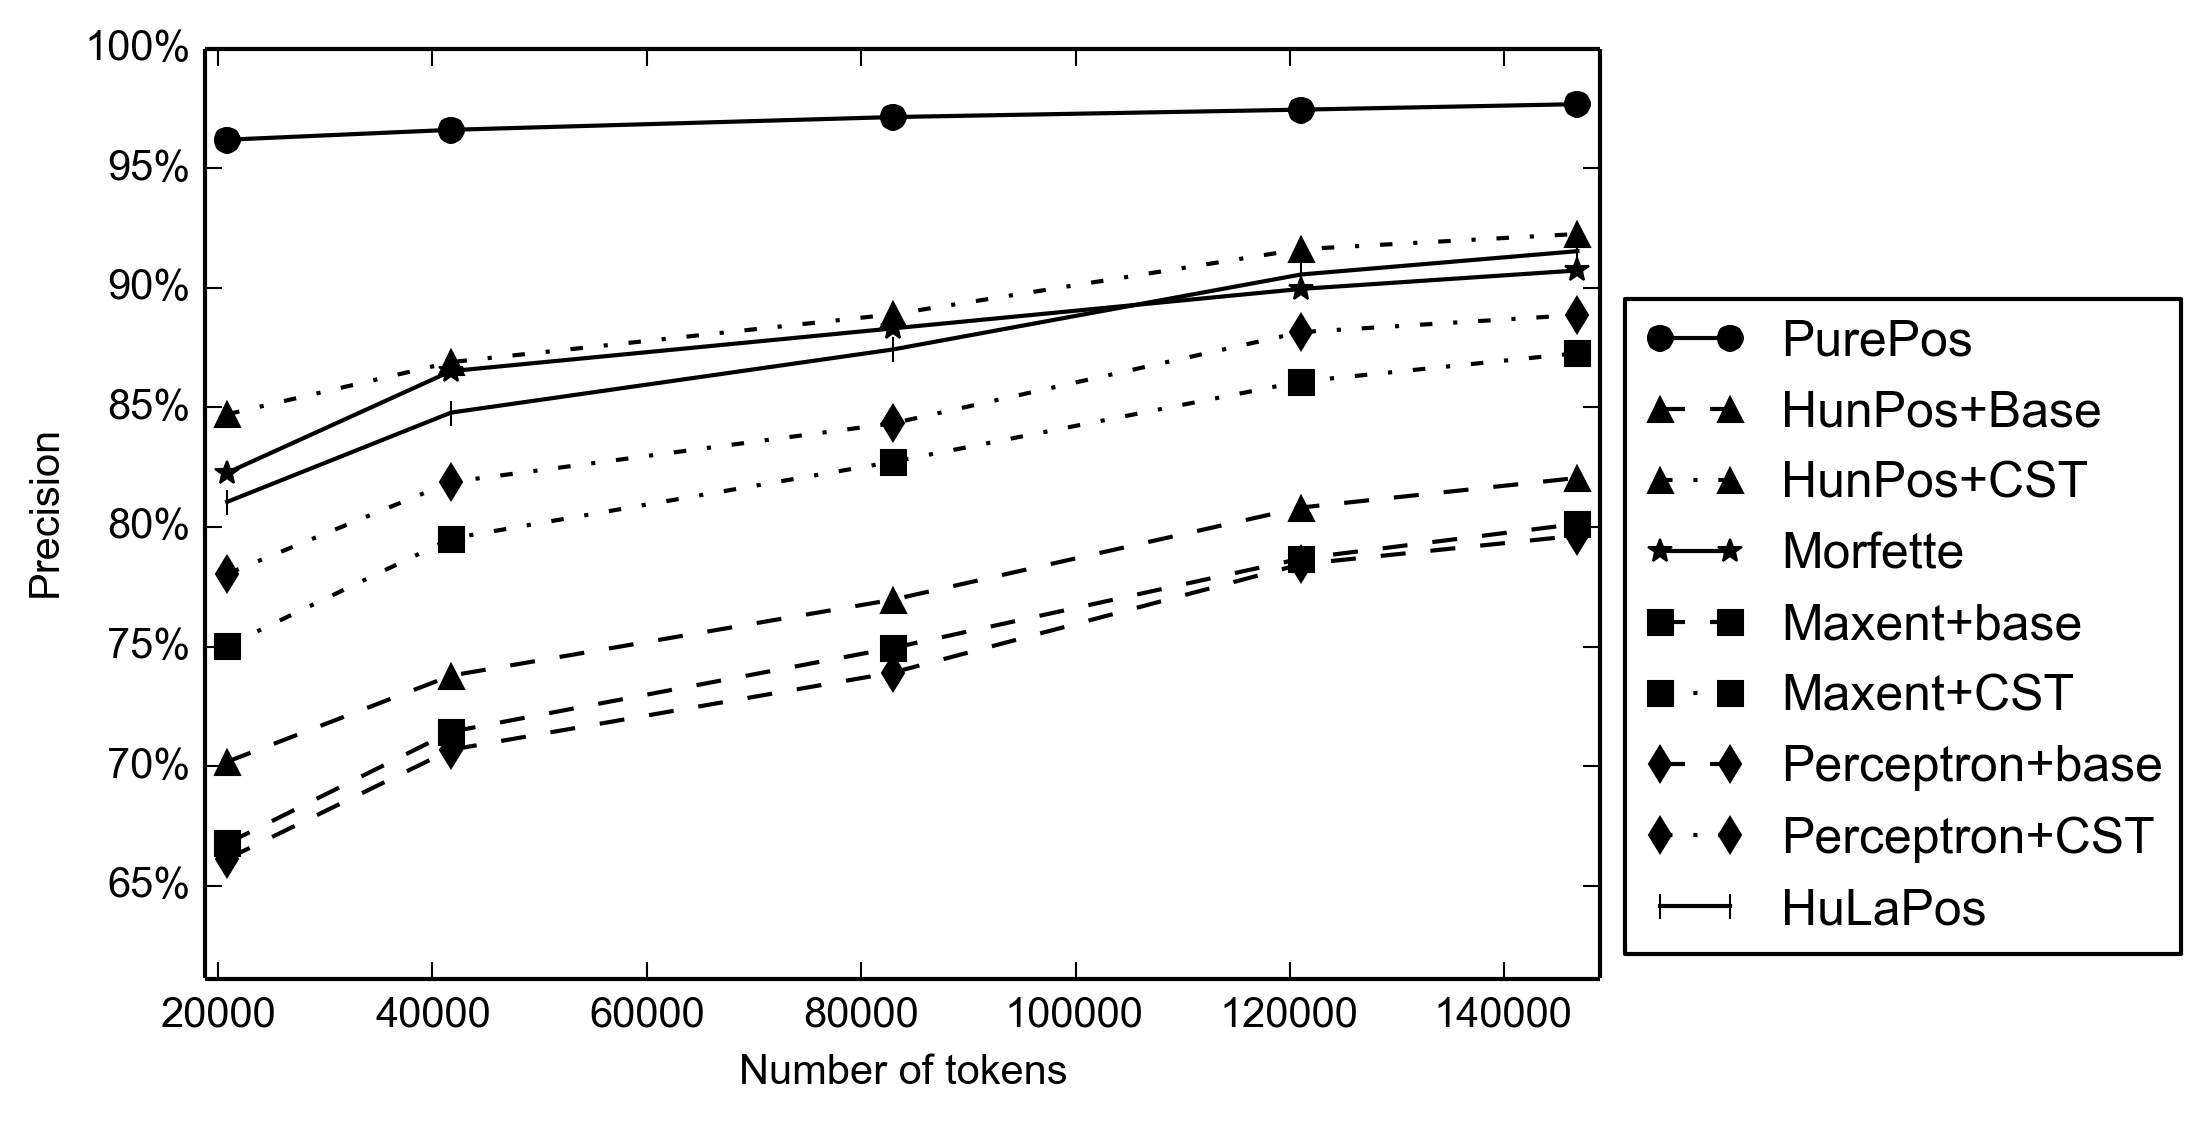
\includegraphics[width=1\textwidth]{MorphTagging/humor_token.png}
  \caption{Learning curves (regarding token accuracy) of full morphological taggers on the Szeged Corpus (using Humor labels)}
  \label{fig:humor-token}
\end{figure}

Figures \ref{fig:msd-token} and \ref{fig:humor-token} present the morphological tagging accuracies of the systems depending on the number of tokens in the training corpus. 
Results are in accordance with conclusions of our previous experiments, however the differences are higher. 
Further on, these also confirm the effectiveness of the hybrid approach in less-resourced scenarios.

\begin{figure}[H]
  \centering
  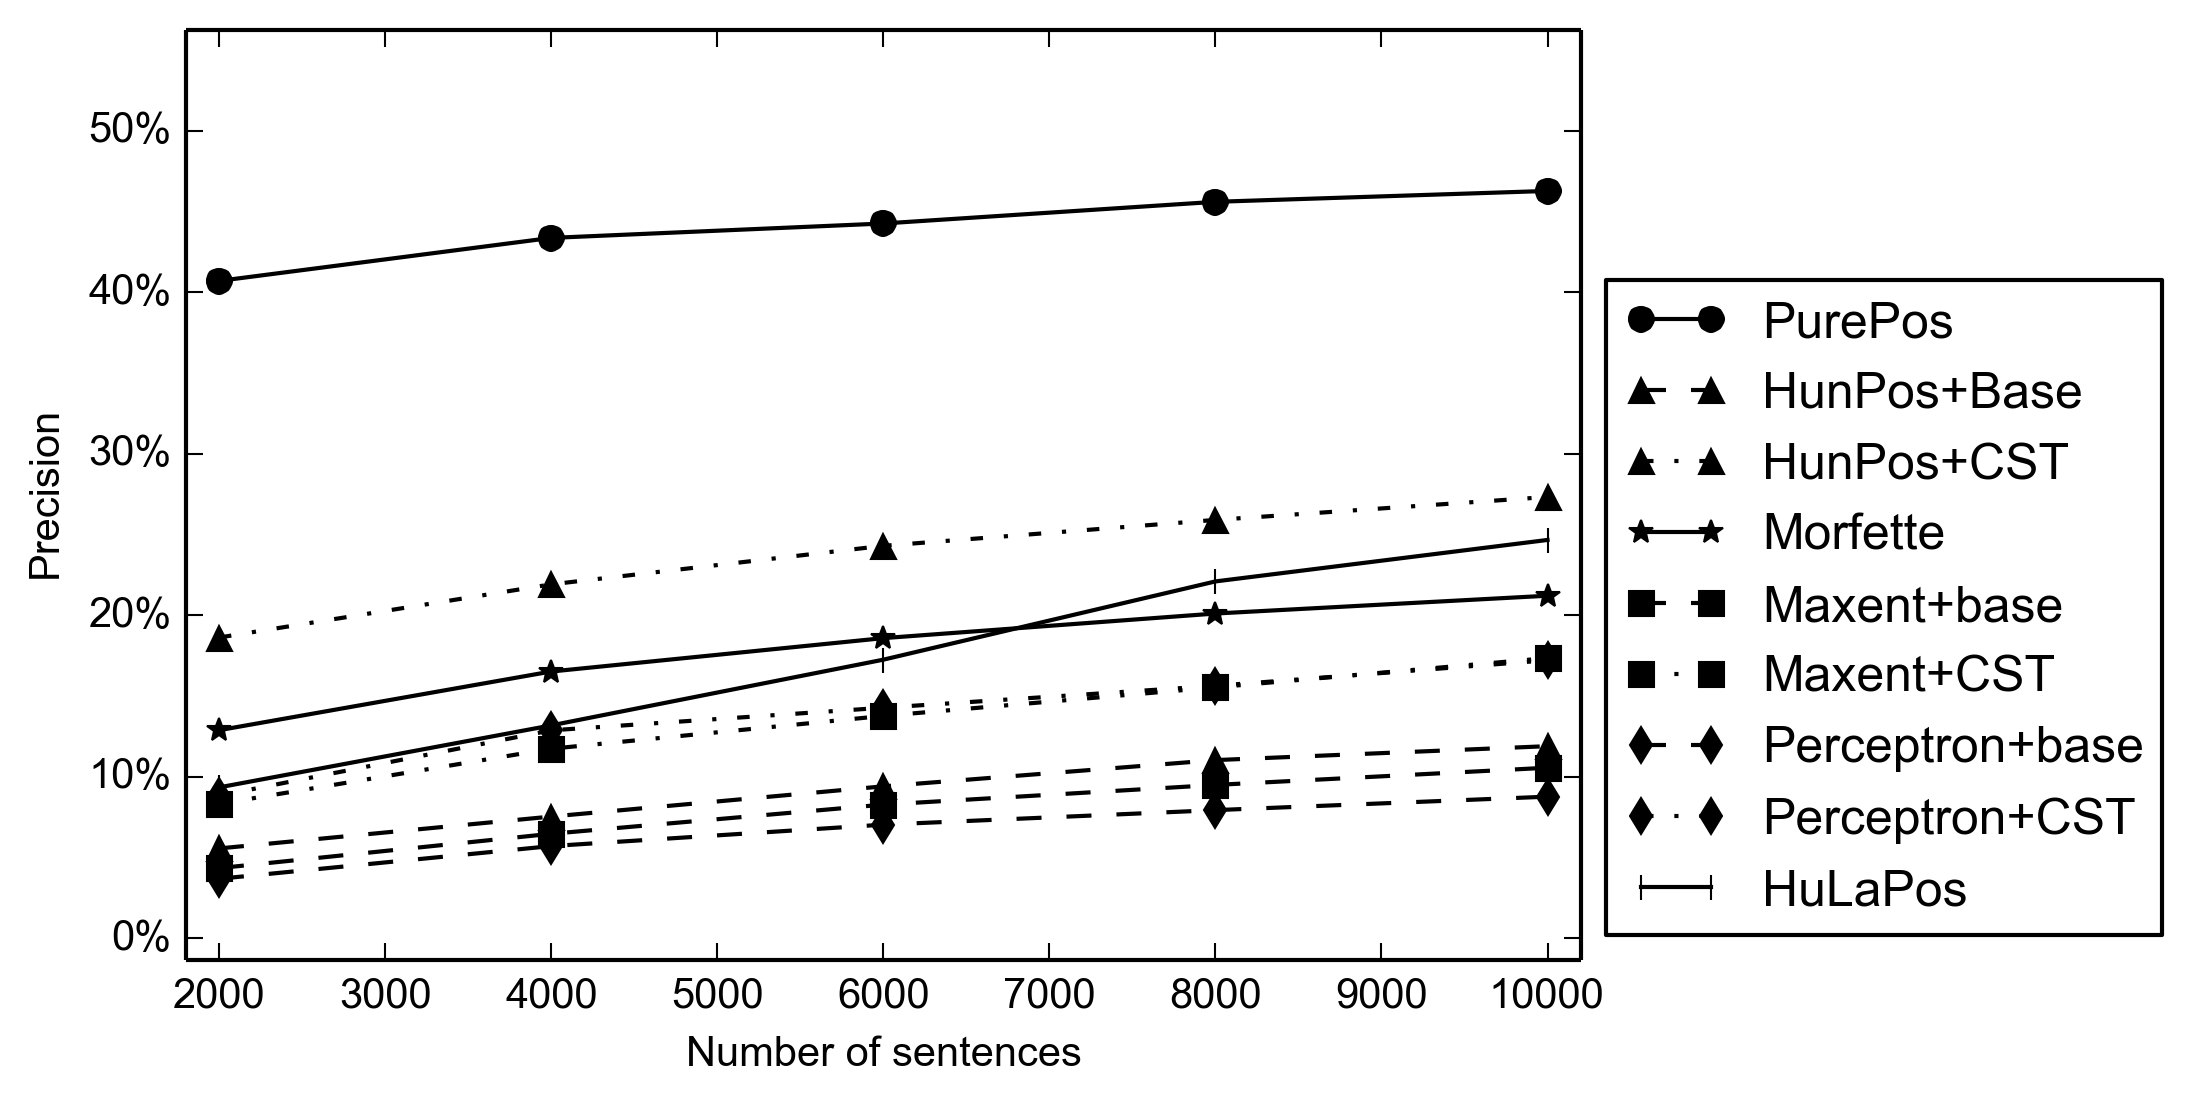
\includegraphics[width=1\textwidth]{MorphTagging/msd_sent.png} 
  \caption{Learning curves (regarding sentence accuracy) of full morphological taggers on the Szeged Corpus (using MSD labels)}
  \label{fig:msd-sent}
\end{figure}

\begin{figure}[H]
  \centering
  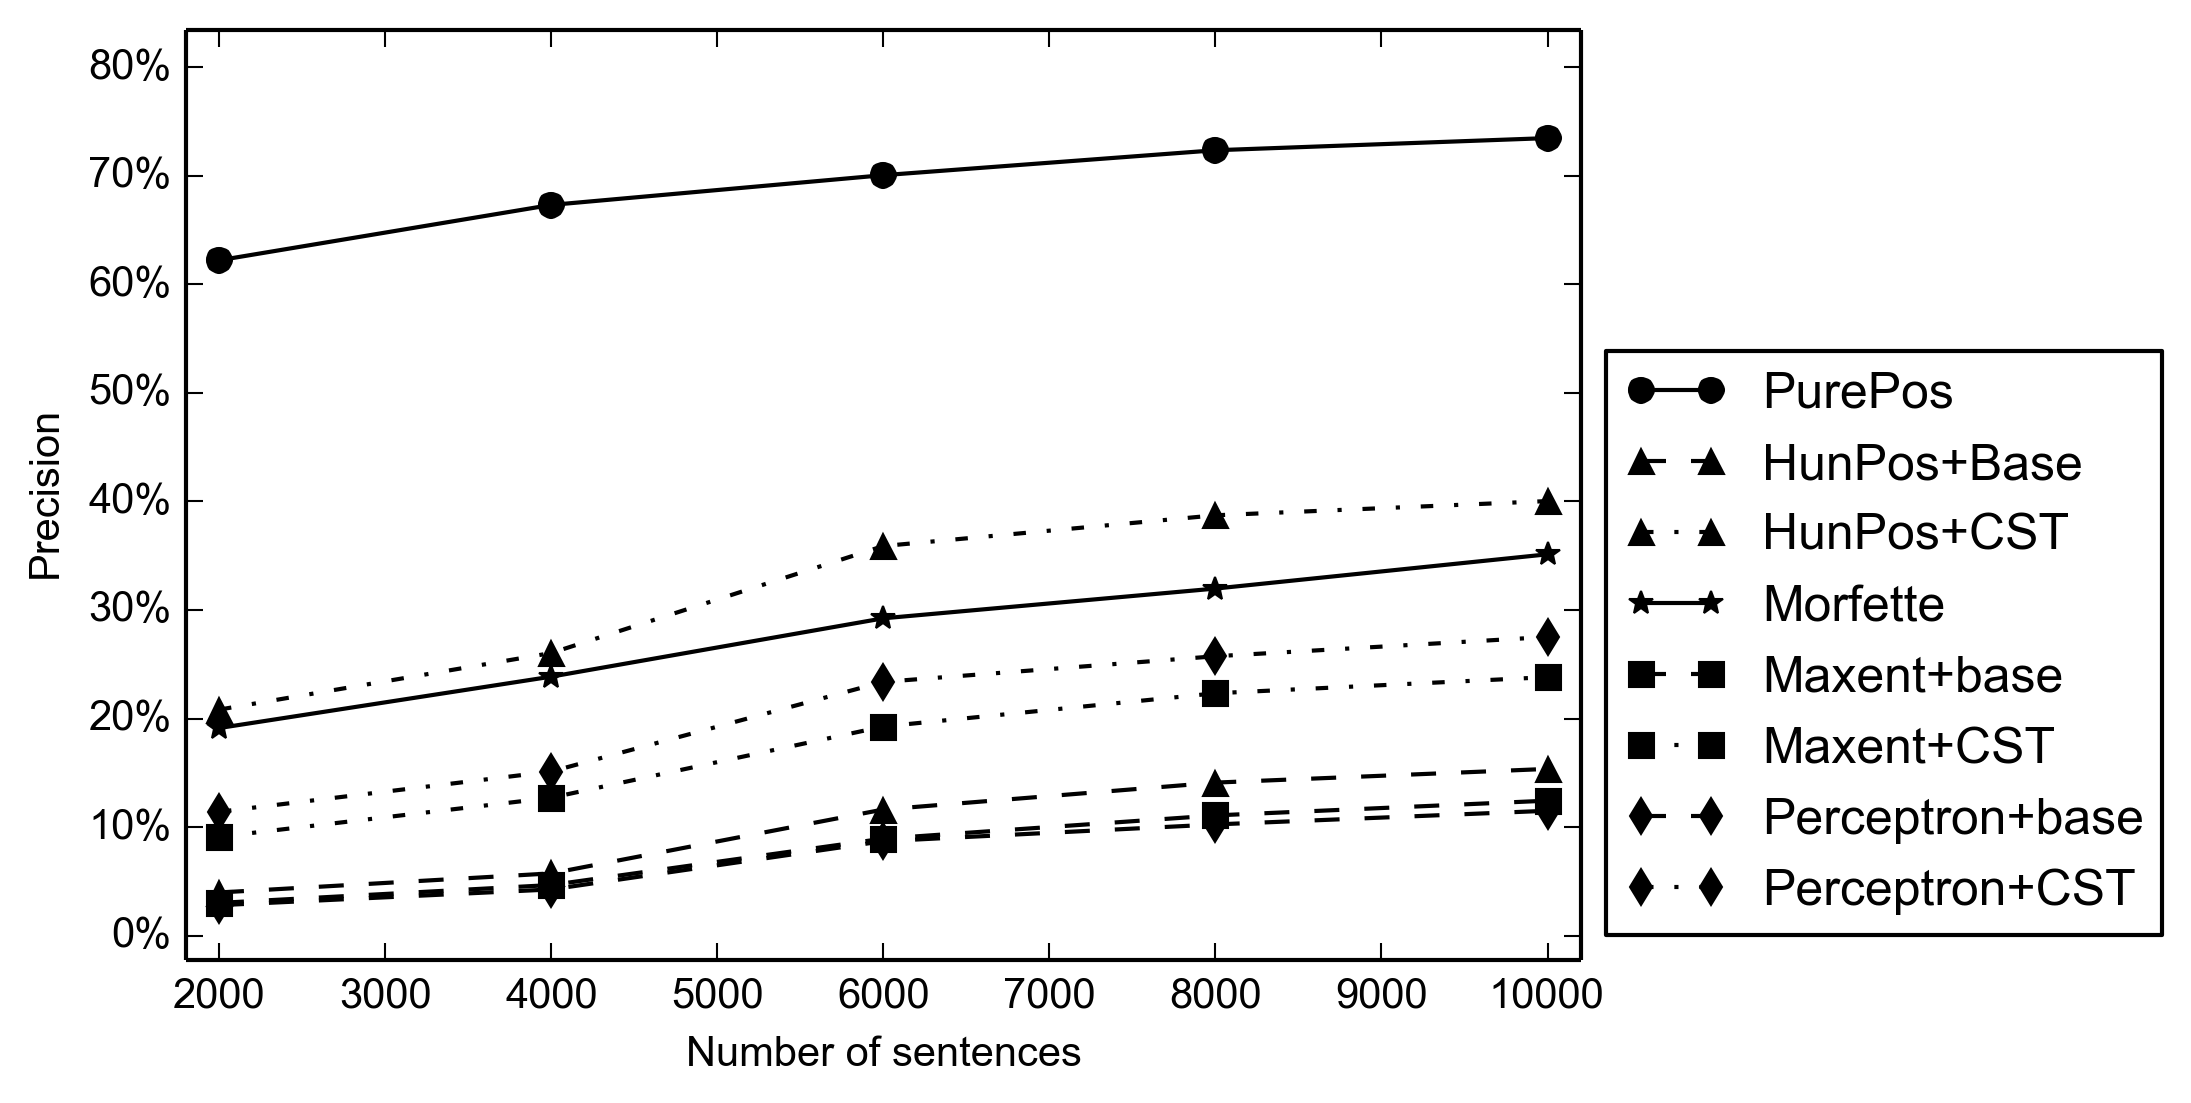
\includegraphics[width=1\textwidth]{MorphTagging/humor_sent.png}
  \caption{Learning curves (regarding sentence accuracy) of full morphological taggers on the Szeged Corpus (using Humor labels)}
  \label{fig:humor-sent}
\end{figure}

Next, if we compare (cf. Figures \ref{fig:msd-sent} and \ref{fig:humor-sent}) full sentence precisions, the gap between taggers are much more emphasized. 
For example, having only 2000 sentences for training (with MSD tags) the proposed algorithm results in 40.71\% sentence precision compared to the second best of 18.62\%.
All in all, the architecture of PurePos allows producing accurate annotations when the amount of training data is limited. 

\subsubsection{The case of Middle- Old-Hungarian}
\label{sec:oldhungarian}

Next, we present a tagging task showing the effectiveness of all hybrid components of PurePos. 
In a project~\cite{Novak2013} aiming at the creation of an annotated corpus of Middle Hungarian texts, an adapted version of the Hungarian Humor morphological analyzer was used. 
This tool was originally made to annotate contemporary Hungarian, but the grammar and lexicon were modified to handle morphological constructions existed in Middle Hungarian but have since disappeared from the language. 
In the experiments described here, we used a manually checked disambiguated portion of this corpus. The data was labeled using a rich variant of the Humor tagset having cardinality over a thousand.

\begin{table}[H]
\centering
\caption{Characteristics of the used corpus}\label{tab:oldhun-corpus}
\begin{tabular}{l r r r}
\hline
& Training & Dev. & Test \\
\hline
Documents & 140 & 20 & 30 \\
Clauses & 12355 & 2731 & 2484 \\
Tokens & 59926 & 12656 &  11763\\
\hline
\end{tabular}
\end{table}

We split the corpus into three parts (see Table \ref{tab:oldhun-corpus}). 
The tagger was trained on the biggest one, hybridization and adaptation methods were developed on a separate development subcorpus, while final evaluation was done on the test set.
We used again precision as an evaluation metric, but unambiguous punctuation tokens were \emph{not} taken into account (in contrast to how taggers are evaluated in general). 
They are ignored because the corpus contains a relatively large amount of punctuation markers which would distort the comparison.
Methods were evaluated twofold: full morphological disambiguation accuracies were calculated for tokens and they were also computed to obtain clause-level precision values.

We used the enhanced trigram-based algorithm derived from HunPos and implemented in PurePos (PP) as a baseline \gls{pos} tagger. 
This basic chain is improved step-by-step investigating the impact of each component.
First, the MA and the new lemmatization method is analyzed on the development set (cf. Table \ref{tab:oldhun-baselines}). 

\begin{table}[H]
\centering
\caption{Baseline disambiguation accuracies on the development set}\label{tab:oldhun-baselines}
\begin{tabular}{l r r r}
\hline
 & Tokens & Clauses \\
\hline
% PP+BL & 93.20\% & 88.99\% & 55.58\% \\
PP+BL  & 88.99\% & 55.58\% \\
% PP+SL & 93.20\% & 89.01\% & 51.78\% \\
% PPM+BL & 97.77\% & 97.22\% & 84.85\% \\
PPM+BL  & 97.22\% & 84.85\% \\
% PPM+SL & 97.77\% & 97.50\% & 85.98\% \\
PP + CL & 92.14\% & 65.40\% \\
PPM + CL & 97.58\% & 86.48\% \\
\hline
\end{tabular}
\end{table}




We compare the \gls{pos} tagging method of PurePos with (PPM) and without the morphological analyzer (PP).
As regards lemmatization, the simple unigram-based (BL) method (cf. Section \ref{sec:purepos-guesser}) is evaluated against the proposed one (CL). 
First, it was found that the usage of a morphological component is indispensable. 
Next, results show that the proposed algorithm yields a significant error rate reduction compared to the baseline. 
This improvement is even more notable  (28.42\% error reduction rate) when a dedicated morphological analyzer is not used.

Experiments are introduced below which exhaust hybrid facilities of PurePos, yielding a more accurate tagger. 
To that end, the development set was utilized to analyze common error types and to develop hypotheses.

\paragraph{Mapping of tags}

In contrast to other Hungarian annotation projects, the tag set of the historical corpus distinguishes verb forms that have a verbal prefix from those that do not, because this is a distinction important for researchers interested in syntax.\footnote{Hungarian verbal prefixes or particles behave similarly to separable verbal prefixes in most Germanic languages: they usually form a single orthographic word with the verb they modify, however, they are separated in certain syntactic constructions.} 
This practically doubles the number of verb tags\footnote{320 different verb tags occur in the corpus excluding verb prefix vs. no verb prefix distinction. This is just a fraction of the theoretically possible tags.}, which results in data sparseness problems for the tagger. 
In case of a never encountered label having a verbal prefix marking, one can calculate probability estimates for that tag by mapping it to one without a verbal prefix. 
This solution is viable, since the distribution of prefixed and non-prefixed verbs largely overlap. 
Applying this enhancement (TM), we could increase the accuracy of the system on the development set (to 86.53\% clause level precision).

\paragraph{Preprocessing}

Another point of improvement is to filter analyses of Humor (FI). 
Exploiting the development set, a preprocessing script was set up which has five simple rules. 
Three of them catches the tagging of frequent phrases such as \emph{az a} `that' in which \emph{az} must be a pronoun. 
Further on, two domain specific lexicons were employed to correct the erroneous annotation of proper names that coincide with frequent common nouns or adjectives. 
Using these correction rules the overall performance on the development set was further raised to 86.77\% clause accuracy.


%%%%%%%%%%%%%%%%%%%%%%%%%%%%%%%%%%%%%%%%%%%%%%%%%%%%%%%%%%%%%%%%%%%%

\paragraph{$k$-best output}
The $k$-best output of the tagger can either be used as a representation to apply upstream grammatical filters to or as candidates for alternative input to higher levels of processing. 
Five-best output for our test corpus has yielded an upper limit for attainable clause accuracy of 94.32\% (on the development set). 
While it is not directly comparable with the ones above, this feature could e.g. be used by syntactic parsers.


\begin{table}[H]
\centering
\caption{Disambiguation accuracies of the hybrid tool on the test set}
\label{tab:oldhun-test}
\begin{tabular}{l r r r}
\hline
 & Full & Clauses  \\
\hline
Baseline  & 89.47\% & 55.07\% \\
PurePos  & 96.48\% & 80.95\% \\
+TM  & 96.51\% & 81.17\% \\
+FI  & 96.60\% & 81.55\% \\
+ all  & 96.63\% & 81.77\% \\
+ all with \emph{k}-best  & 98.66 \% & 92.30\% \\
\hline
\end{tabular}
\end{table}
 
Enhancements are validated measuring improvements on the test set.
Data in Table \ref{tab:oldhun-test} shows that each linguistic component significantly improves the overall chain.
Further on, using the $5$-best output sequence of the tagger provide us much more golden annotations. 
These are available for 92.30\% of the clauses and for 98.66\% of the tokens.

All in all, we have shown that one can further increase the tagging accuracy by employing the hybrid facilities of PurePos. 
In this work, rules has been employed to preprocess analyses candidates. 
Further on, unseen tags are mapped to previously seen ones successfully. 
Finally, we have shown that the 5-best output contain more golden annotations that can either be used as a representation to apply upstream grammatical filters to or as candidates for alternative input to higher levels of processing.


